\section{Giới thiệu đề tài}
\subsection{Thực trạng}
\subsubsection{Thực trạng chung}
\indent \indent Trong bối cảnh xã hội hiện nay, cùng với sự phát triển mạnh mẽ của Internet và các nền tảng thương mại điện tử, việc mua vé sự kiện trực tuyến đang trở thành xu hướng phổ biến. Người dùng có thể dễ dàng tham gia các chương trình ca nhạc, hội nghị, lễ hội hoặc workshop chỉ với vài thao tác trên trình duyệt.\\
\indent Theo báo cáo của The Business Research Company (2024), quy mô thị trường đặt vé sự kiện trực tuyến toàn cầu đạt 50,97 tỷ USD vào năm 2024 và dự kiến sẽ tăng lên 67,89 tỷ USD vào năm 2029, với tốc độ tăng trưởng trung bình (CAGR) 6,4\%/năm.\\
\indent Tại Việt Nam, theo 6W Research (2025), thị trường đặt vé sự kiện trực tuyến được dự báo tăng trưởng mạnh mẽ trong giai đoạn 2025–2031, nhờ sự phát triển của hạ tầng thanh toán điện tử và tỷ lệ người dùng Internet cao. \\
\indent Với những lợi ích thiết thực đó, hình thức đặt vé sự kiện trực tuyến ngày càng được hệ thống rộng rãi trong nhiều lĩnh vực khác nhau. Chẳng hạn, trong ngành giải trí, các nền tảng đặt vé hỗ trợ người dùng mua vé concert, phim, lễ hội chỉ với vài thao tác trên trình duyệt; trong giáo dục, các trường học có thể áp dụng hệ thống để tổ chức và quản lý các sự kiện lớn như Job Fair, cuộc thi học thuật, hội nghị hay đại hội,... thay vì sử dụng các biểu mẫu đăng ký truyền thống. \\
\indent Việc số hóa quy trình bán vé không chỉ mang lại trải nghiệm thuận tiện và minh bạch cho người dùng, mà còn giúp Ban tổ chức tiết kiệm thời gian, giảm chi phí nhân sự và kiểm soát tốt hơn doanh thu cũng như lượng người tham dự.\\
\indent Nhóm thực hiện đã tiến hành một khảo sát nhỏ trong các hội nhóm mạng xã hội dành cho người thường xuyên tham gia sự kiện, kết quả thu được:
\begin{itemize}
    \item[-] 86\% người được hỏi cho rằng họ ưu tiên mua vé online thay vì mua tại quầy.
    \item[-] 31\% cho rằng các nền tảng hiện tại khó thao tác hoặc giao diện chưa thân thiện.
    \item[-] 78\% nói rằng liên hệ với Ban tổ chức để được hỗ trợ còn nhiều khó khăn.
    \item[-] 62\% mong muốn có chức năng đánh giá và phản hồi sau sự kiện.
\end{itemize}
\begin{figure}[H]
    \centering
    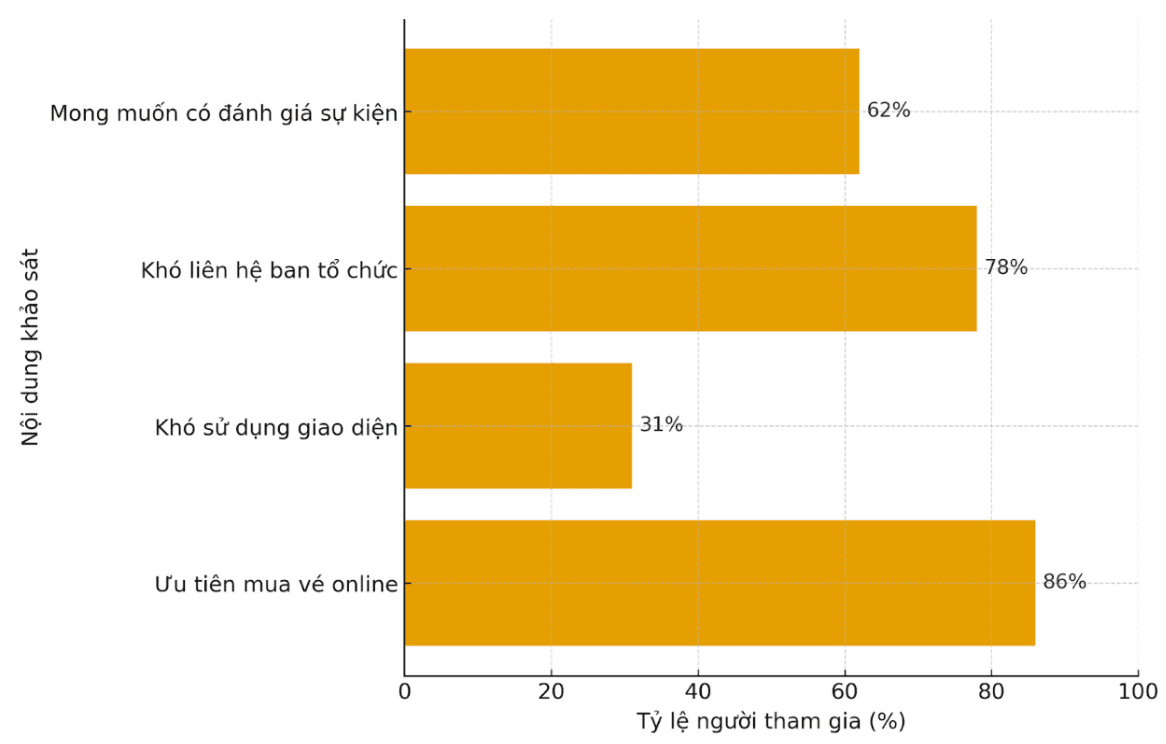
\includegraphics[width=0.7\textwidth]{Images/KhaoSat.png}
    \vspace{10pt}
    \caption{Kết quả khảo sát dành cho người tham gia sự kiện}
    \label{fig:khao_sat}
\end{figure}
\indent \indent Các kết quả này cho thấy nhu cầu có một nền tảng đặt vé sự kiện đơn giản, tiện lợi, bảo mật và có tính tương tác cao là vô cùng cần thiết, đặc biệt trong bối cảnh Việt Nam đang đẩy mạnh chuyển đổi số trong lĩnh vực giải trí và dịch vụ.
\subsubsection{Thực trạng các hệ thống hiện có}
\indent \indent Hiện nay, tại Việt Nam có nhiều nền tảng cung cấp dịch vụ đặt vé trực tuyến như TicketBox, VnTicket, Ticketgo,… Tuy nhiên, qua khảo sát và phân tích, nhóm nhận thấy các hệ thống này còn tồn tại nhiều hạn chế:
\begin{itemize}
    \item[1.] \textbf{Đối với người dùng:}
    \begin{itemize}
        \item[-] Hầu hết các hệ thống chỉ hỗ trợ tìm kiếm bằng văn bản, chưa có tìm kiếm bằng giọng nói (voice search) – trong khi theo Think with Google, hơn 27\% người dùng Việt Nam cho biết họ thường xuyên sử dụng tìm kiếm bằng giọng nói trên thiết bị di động.
        \item[-] Các nền tảng lớn không hỗ trợ trao đổi trực tiếp với Ban tổ chức, gây khó khăn khi cần hỗ trợ đổi, hủy vé hoặc khi có sự cố.
        \item[-] Việc đánh giá, nhận xét sau sự kiện chưa được chú trọng, khiến người tham gia không có kênh phản hồi chính thức và Ban tổ chức không có cơ sở cải thiện chất lượng dịch vụ.
    \end{itemize}
    \item[2.] \textbf{Đối với Ban tổ chức sự kiện:}
    \begin{itemize}
        \item[-] Khó quản lý danh sách khách hàng và theo dõi hiệu quả bán vé.
        \item[-]Thiếu công cụ chat hoặc phản hồi tin nhắn của người dùng trong thời gian thực.
    \end{itemize}
\end{itemize}
\indent \indent Từ các kết quả khảo sát và thống kê trên, nhóm nhận thấy cần phát triển một hệ thống web đặt vé sự kiện trực tuyến – MyTicket có thể khắc phục các hạn chế hiện tại, tập trung vào trải nghiệm người dùng, tính tiện lợi và khả năng tương tác hai chiều giữa người tham dự và Ban tổ chức.
\subsection{Mục tiêu của đề tài}
\indent \indent Mục tiêu chính của đề tài là xây dựng hệ thống web đặt vé sự kiện trực tuyến – MyTicket, giúp người dùng dễ dàng tìm kiếm, mua và quản lý vé, đồng thời hỗ trợ Ban tổ chức và quản trị viên trong việc giám sát, phản hồi và nâng cao chất lượng sự kiện.\\
\indent Các mục tiêu cụ thể gồm:
\begin{itemize}
    \item[1.] \textbf{Đối với người dùng:}
    \begin{itemize}
        \item[-] Tìm kiếm sự kiện bằng văn bản hoặc giọng nói.
        \item[-] Đặt vé trực tuyến và thanh toán an toàn qua ví điện tử MoMo.
        \item[-] Xem lại danh sách sự kiện đã mua vé.
        \item[-] Chat trực tiếp với Ban tổ chức hoặc admin hệ thống để được hỗ trợ.
        \item[-] Đánh giá và nhận xét sự kiện sau khi tham dự.
    \end{itemize}
    \item[2.] \textbf{Đối với Ban tổ chức}
    \begin{itemize}
        \item[-] Theo dõi danh sách sự kiện do đơn vị mình tổ chức đã và đang được đăng tải lên hệ thống.
        \item[-] Phản hồi tin nhắn người dùng ngay trong hệ thống.
    \end{itemize}
    \item[3.] \textbf{Đối với quản trị viên:}
    \begin{itemize}
        \item[-] Quản lý danh sách sự kiện và đơn vị tổ chức.
        \item[-] Tạo hoặc chỉnh sửa thông tin một sự kiện hay một đơn vị tổ chức cụ thể.
        \item[-] Phản hồi các tin nhắn của người dùng
    \end{itemize}
\end{itemize}
\subsection{Phạm vi đề tài}
\begin{itemize}
    \item[-] Đề tài tập trung phát triển phiên bản web của hệ thống, chưa triển khai trên thiết bị di động.
    \item[-] Hệ thống hỗ trợ phương thức thanh toán duy nhất qua ví điện tử MoMo, có thể nhận chuyển khoản từ hầu hết ngân hàng.
    \item[-] Các tính năng chính được hiện thực bao gồm:
    \begin{itemize}
        \item[1.] Đăng ký, đăng nhập, xác thực người dùng.
        \item[2.] Tìm kiếm sự kiện (bằng văn bản và bằng giọng nói).
        \item[3.] Đặt vé và thanh toán trực tuyến.
        \item[4.] Chat trực tiếp giữa người dùng và Ban tổ chức.
        \item[5.] Đánh giá và phản hồi sự kiện sau khi tham dự.
    \end{itemize}
\end{itemize}
